\documentclass[../main.tex]{subfiles}
\begin{document}
\setchapterstyle{kao}
\setchapterpreamble[u]{\margintoc}
\setchapterimage[6.5cm]{Images/emint.jpg}
\chapter[Electromagnetic Interactions]{Electromagnetic Interactions\footnotemark[0]}
\labch{EMInteractions}
\section{Quantum Electrodynamics}
We are now interested in studying the QED interaction between the electromagnetic field and spin $\frac{1}{2}$ field. In the classical theory, this interaction is described by the minimal substitution $P^\mu\xrightarrow[]{}P^\mu-eA^\mu$ while in quantum mechanics we have $i\partial^\mu\xrightarrow[]{}i\partial^\mu-eA^\mu$. The theory which describes photons and electrons is obtained by combining the Maxwell Lagrangian [\refeq{MaxwellLagrangian}] and the Dirac Lagrangian [\refeq{DiracLagrangian}]:
\[
\pazocal{L}_0=-\frac{1}{4}F_{\mu\nu}F^{\mu\nu}+\bar{\Psi}(i\slashed{\partial}-m)\Psi
\]
This is for a free particle Lagrangian, if we want the interacting one we have to include the minimal substitution:
\begin{align*}
\pazocal{L}&=\bar{\Psi}(i\slashed{\partial}-e\slashed{A}-m)\Psi-\frac{1}{4}F_{\mu\nu}F^{\mu\nu}\\
&=\bar{\Psi}(i\slashed{\partial}-m)\Psi-\frac{1}{4}F_{\mu\nu}F^{\mu\nu}-eA_\mu\bar{\Psi}\gamma^\mu\Psi\\
&=\pazocal{L}_0+\pazocal{L}_{int}
\end{align*}
Let's take now a gauge transformation $A^\mu\xrightarrow[]{}A'^\mu=A^\mu+\partial^\mu\Lambda(x)$ and see how the Lagrangian $\pazocal{L}$ behaves under such transformation:
\begin{align*}
\pazocal{L}\xrightarrow[]{}\pazocal{L}'&=\pazocal{L}_0-eA_\mu\bar{\Psi}\gamma^\mu\Psi-e\bar{\Psi}\gamma^\mu\Psi\partial_\mu\Lambda(x)\\
&=\pazocal{L}-e\bar{\Psi}\gamma^\mu\Psi\partial_\mu\Lambda(x)
\end{align*}
Therefore, $\pazocal{L}$ is \textbf{not invariant} under gauge transformation but there is still a symmetry: we know that the Dirac Lagrangian is invariant under a global phase transformation so we could try to use a transformation depending on the point, such that:
\[
\Psi(x)\xrightarrow[]{}\Psi'(x)=e^{-ie\Lambda(x)}\Psi(x)
\]
What we obtain for $\pazocal{L}$ is:
\begin{align*}
\pazocal{L}\xrightarrow[]{}\pazocal{L}'&=\bar{\Psi}e^{ie\Lambda(x)}(i\slashed{\partial}-m)e^{-ie\Lambda(x)}\Psi-\frac{1}{4}F_{\mu\nu}F^{\mu\nu}-eA_\mu\bar{\Psi}\gamma^\mu\Psi\\
&=\bar{\Psi}(i\slashed{\partial}-m)\Psi+\bar{\Psi}e^{ie\Lambda(x)}e\gamma^\mu\partial_\mu\Lambda(x)e^{-ie\Lambda(x)}\Psi-\frac{1}{4}F_{\mu\nu}F^{\mu\nu}-eA_\mu\bar{\Psi}\gamma^\mu\Psi\\
&=\pazocal{L}+e\bar{\Psi}\gamma^\mu\Psi\partial_\mu\Lambda(x)
\end{align*}
If we use the same $\Lambda$ of the gauge, then $\pazocal{L}$ is invariant under:
\[
\left\{
\begin{aligned}
A^\mu&\xrightarrow[]{}A'^\mu=A^\mu+\partial^\mu\Lambda(x)\\
\Psi&\xrightarrow[]{}\Psi'=e^{-ie\Lambda(x)}\Psi
\end{aligned}
\right.
\]
It is possible now to introduce the \textbf{covariant derivative} $D^\mu:=\partial^\mu+ieA^\mu$ and we show that this is actually covariant, i.e. it transforms like the field:
\begin{align*}
D^\mu\Psi\xrightarrow[]{}D'\mu\Psi'&=[\partial^\mu+ieA^\mu+ie\partial^\mu\Lambda(x)]e^{-ie\Lambda(x)}\Psi\\
&=\cancel{-ie\partial^\mu\Lambda(x)e^{-ie\Lambda(x)}\Psi}+e^{-ie\Lambda(x)}(\partial^\mu\Psi+ieA^\mu\Psi)+\cancel{ie\partial^\mu\Lambda(x)e^{-ie\Lambda(x)}\Psi}\\
&=e^{-ie\Lambda(x)}D^\mu\Psi \quad \checkmark
\end{align*}
Now, we can express $\pazocal{L}$ in terms of the covariant derivative to obtain a more compact form:
\[
\pazocal{L}=\bar{\Psi}(i\slashed{D}-m)\Psi-\frac{1}{4}F_{\mu\nu}F^{\mu\nu}
\]
\subsection{Quantization of the Lagrangian}
We have seen that $\pazocal{L}=\pazocal{L}_0+\pazocal{L}_{int}$, i.e. it is a function of the Dirac field and the electromagnetic field. We can construct the conjugated momenta in order to impose the usual commutation relations:
\[
\left\{
\begin{aligned}
\pi_\Psi&=\frac{\partial\pazocal{L}}{\partial\Dot{\Psi}}=\frac{\partial\pazocal{L}_0}{\partial\Dot{\Psi}}\\
\pi^\mu&=\frac{\partial\pazocal{L}}{\partial\Dot{A}_\mu}=\frac{\partial\pazocal{L}_0}{\partial\Dot{A}_\mu}=F^{\mu0}-\eta^{\mu0}(\partial_\lambda A^\lambda)
\end{aligned}
\right.
\]
Once again, we impose the commutation relations:
\[
\left\{
\begin{aligned}
[A_\mu(\underline{x},t),\pi_\nu(\underline{y},t)]&=i\eta_{\mu\nu}\delta^3(\underline{x}-\underline{y})\\
[\Psi(\underline{x},t)\pi_\Psi(\underline{y},t)]_+&=i\delta^3(\underline{x}-\underline{y})
\end{aligned}
\right.
\]
Finally, we can move to the Hamiltonian and we get:
\[
H=\pi_i\Dot{\Phi}^i-\pazocal{L}_0-\pazocal{L}_{int}=H_0+H_{int}
\]
\section{Time evolution}
Let's consider a set of particles in a state $\phi_i$ at $t=-\infty$ and $\phi_f$ at $t=+\infty$. In the Schr\"odinger's picture, the time evolution is given by:
\[
i\frac{\partial}{\partial t}\ket{\phi_s(t)}=(H_s^0+H_s^{int})\ket{\phi_s(t)}
\]
We can define $S\ket{\phi(-\infty)}:=\ket{\phi(+\infty)}$ so that we have:
\[
\lim_{t\to+\infty}\bra{\phi_f}\ket{\phi(t)}=\bra{\phi_f}S\ket{\phi_i}=S_{fi}
\]
In the interaction picture, we have $\ket{\phi_I}=e^{iH_s^0t}\ket{\phi_s(t)}$, therefore the Schr\"odinger's time evolution becomes:
\begin{align*}
i\frac{\partial}{\partial t}\ket{\phi_I}&=i\frac{\partial}{\partial t}\left(e^{iH_s^0t}\ket{\phi_s(t)}\right)\\
&=-H_s^0e^{iH_s^0t}\ket{\phi_s(t)}+e^{iH_s^0t}i\frac{\partial}{\partial t}\ket{\phi_s(t)}\\
&=\cancel{-H_s^0e^{iH_s^0t}\ket{\phi_s(t)}}+e^{iH_s^0t}(\cancel{H_s^0}+H_s^{int})\ket{\phi_s(t)}\\
&=e^{iH_s^0t}H_s^{int}e^{-iH_s^0t}\ket{\phi_I}=H_I\ket{\phi_I}
\end{align*}
By integrating this in $t$, we obtain:
\begin{align*}
\phi(t)&=\phi(-\infty)-i\int_{-\infty}^tdt_1H_I(t_1){\color{blue}\phi(t_1)}\\
&=\phi(-\infty)-i\int_{-\infty}^tdt_1H_I(t_1){\color{blue}\left[\phi(-\infty)-i\int_{-\infty}^{t_1}dt_2H_I(t_2)\phi(t_2)\right]}\\
&=\phi(-\infty)-i\phi(-\infty)\int_{-\infty}^tdt_1H_I(t_1)+(-i)^2\int_{-\infty}^t\int_{-\infty}^{t_1}dt_1dt_2H_I(t_1)H_I(t_2){\color{green}\phi(t_2)}\\
&=\phi(-\infty)-i\phi(-\infty)\int_{-\infty}^tdt_1H_I(t_1)+(-i)^2\int_{-\infty}^t\int_{-\infty}^{t_1}dt_1dt_2H_I(t_1)H_I(t_2){\color{green}\left[\phi(-\infty)-i\int_{-\infty}^{t_2}dt_3H_I(t_3)\phi(t_3)\right]}\\
&=\phi(-\infty)-i\phi(-\infty)\int_{-\infty}^tdt_1H_I(t_1)+(-i)^2\phi(-\infty)\int_{-\infty}^t\int_{-\infty}^{t_1}dt_1dt_2H_I(t_1)H_I(t_2)\\
&+(-i)^3\int_{-\infty}^{t}\int_{-\infty}^{t_1}\int_{-\infty}^{t_2}dt_1dt_2dt_3H_I(t_1)H_I(t_2)H_I(t_3)\phi(t_3)
\end{align*}
Where the $t_i$ are defined such that $t>t_1>t_2>\dots>t_n$. After repeating this process for $N$ times, the final result is:
\begin{align*}
\phi(t)&=\phi(-\infty)\left[1+\sum_{n=1}^{N-1}(-i)^n\int_{-\infty}^t\int_{-\infty}^{t_1}\dots\int_{-\infty}^{t_{n-2}}dt_1\dots dt_{n-1}H_I(t_1)\dots H_I(t_{n-1})\right]\\
&+(-i)^N\int_{-\infty}^t\dots\int_{-\infty}^{t_{N-1}}dt_1\dots dt_NH_I(t_1)\dots H_I(t_N)\phi(t_N)
\end{align*}
In the limit $N\to\infty$, we get that $\phi(t_N)\to\phi(-\infty)$ and the final result is:
\[
\phi(t)=\left[1+\sum_{n=1}^\infty(-i)^n\int_{-\infty}^t\int_{-\infty}^{t_1}\dots\int_{-\infty}^{t_{n-1}}dt_1\dots dt_nH_I(t_1)\dots H_I(t_n)\right]\phi(-\infty)
\]
Taking the limit of $t$ going to infinity, we recover:
\[
\lim_{t\to\infty}\phi(t)=\lim_{t\to\infty}[\dots]\phi(-\infty)=S\phi(-\infty)
\]
Considering that we have defined $t_i$ such that $t_1>t_2>\dots>t_n$, it is possible to use the time-ordered product to write $S$ in a more compact form:
\[
S=\sum_{n=0}^\infty\frac{(-i)^n}{n!}\int_{-\infty}^{+\infty}\int_{-\infty}^{+\infty}\dots\int_{-\infty}^{+\infty}dt_1\dots dt_nT[H_I(t_1)H_I(t_2)\dots H_I(t_n)]
\]
The $n!$ comes from the fact that we moved the upper bound of all the integrals to the same time. If we do that, we no longer have only the ordered product but we have to consider all the possible permutations.
\begin{marginfigure}
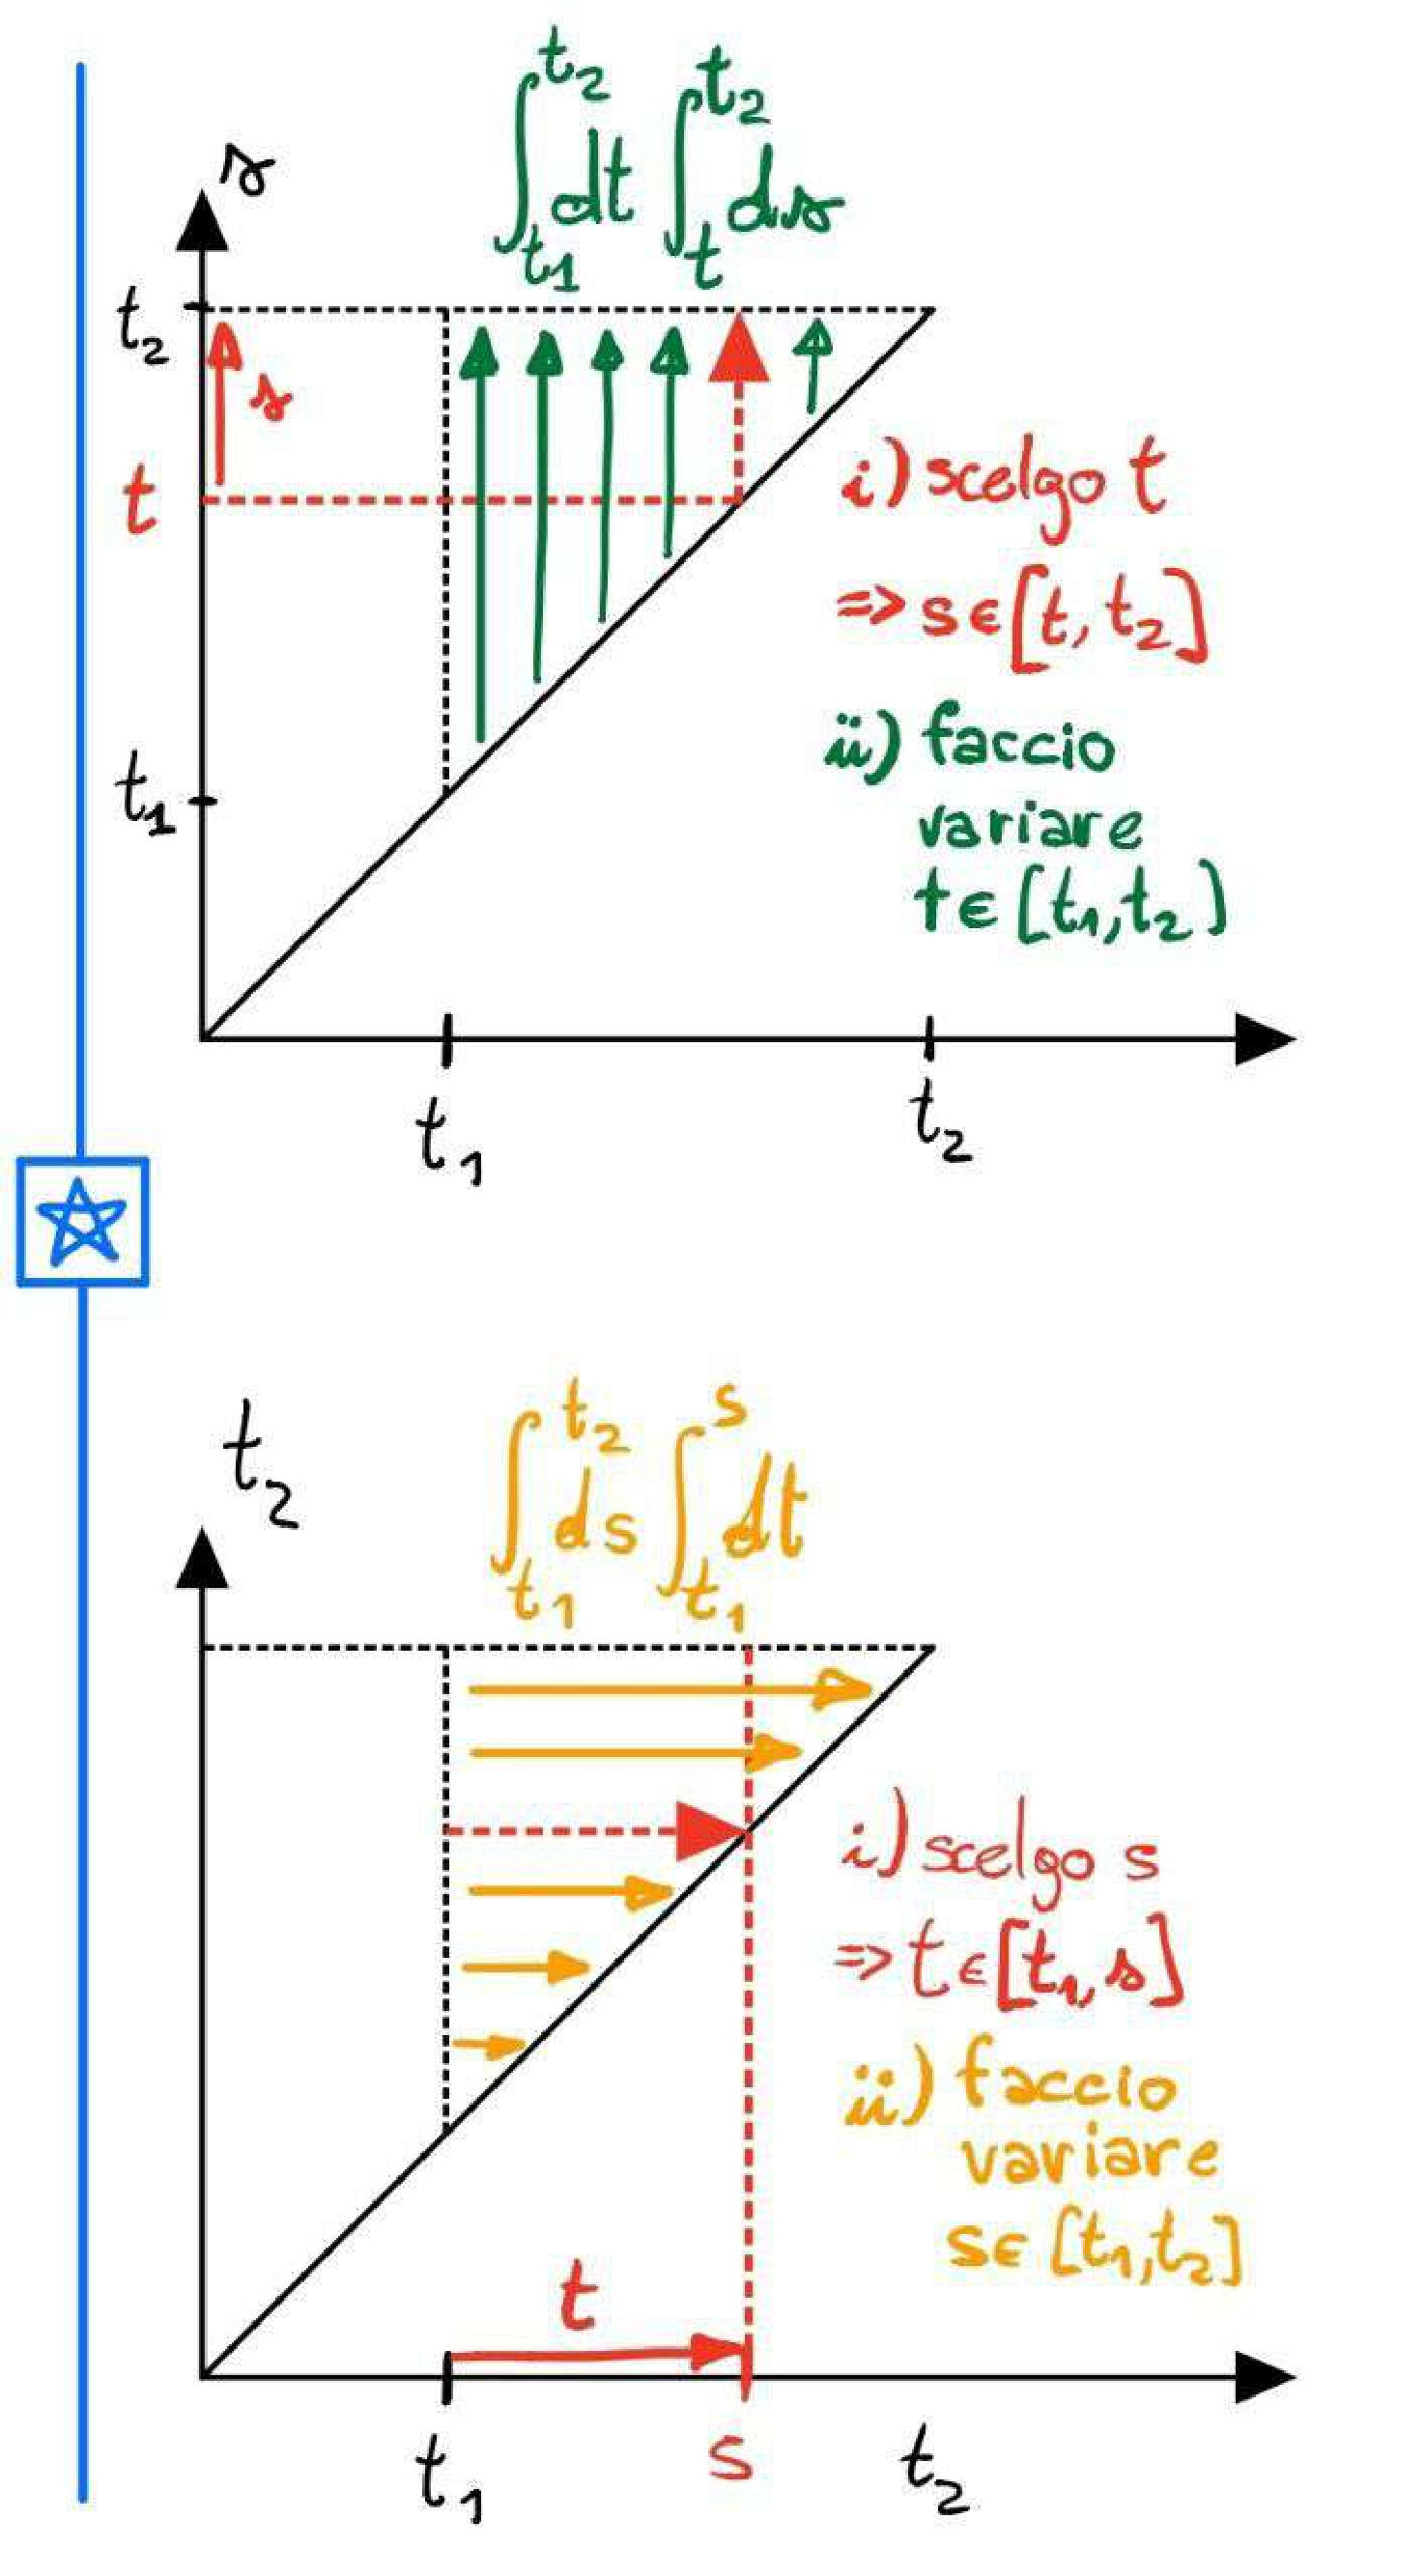
\includegraphics{Images/papaintegrale.pdf}
\caption{Explanation of the change of integral in red. Picture taken from \cite{PapaNotes}.}
\end{marginfigure}
\begin{kaobox}[frametitle=Check]
As a check, we compute the second order term:
\begin{align*}
A_2&=\int_{t_1}^{t_2}dt\int dsT[H(t)H(s)]\\
&=\int_{t_1}^{t_2}dt\left[\int_{t_1}^tdsH(t)H(s)+\int_t^{t_2}dsH(s)H(t)\right]\\
&=\int_{t_1}^{t_2}dt\int_{t_1}^tdsH(t)H(s)+{\color{red}\int_{t_1}^{t_2}dt\int_t^{t_2}ds}H(s)H(t)\\
&=\int_{t_1}^{t_2}dt\int_{t_1}^tdsH(t)H(s)+{\color{red}\int_{t_1}^{t_2}ds\int_{t_1}^sdt}H(s)H(t)\\
&=2!\int_{t_1}^{t_2}dt\int_{t_1}^tdsH(t)H(s) \quad \checkmark
\end{align*}
\end{kaobox}
It is not difficult to see that $S$ is nothing but the series expansion of the exponential, therefore:
\begin{kaobox}[frametitle=Dyson formula]
\[
S=T\left[\exp{-i\int_{-\infty}^{+\infty} dtH_I(t)}\right]
\]
\end{kaobox}
The integral in the exponential can be written as:
\[
\int dtH_I(t)=\int d^4x\pazocal{H}_I=-\int d^4x\pazocal{L}_{int}\Rightarrow S=T\left(\exp{i\int d^4x\pazocal{L}_{int}}\right)
\]
\subsection{Properties of the time-ordered exponential}
\begin{proposition}
\labprop{property1}
The time-ordered product defined above satisfies the following property:
\[
T\left(e^{\int_{t_1}^{t_3}dtO(t)}\right)=T\left(e^{\int_{t_2}^{t_3}dtO(t)}\right)T\left(e^{\int_{t_1}^{t_2}dtO(t)}\right) \quad \text{with } t_1<t_2<t_3
\]
\end{proposition}
\begin{proof}
\begin{align*}
T\left(\int_{t_1}^{t_3}dtO(t)\right)^n&=\int_{t_1}^{t_3}ds_1\dots ds_nT[O(s_1)\dots O(s_n)]\\
&=\left(\int_{t_2}^{t_3}+\int_{t_1}^{t_2}\right)ds_1\dots\left(\int_{t_2}^{t_3}+\int_{t_1}^{t_2}\right)ds_nT[O(s_1)\dots O(s_n)]\\
&=\sum_{k=0}^n\frac{n!}{(n-k)!k!}\underbrace{\int_{t_2}^{t_3}\dots\int_{t_2}^{t_3}}_{n-k \text{ times}}ds_1\dots ds_{n-k}\underbrace{\int_{t_1}^{t_2}\dots\int_{t_1}^{t_2}}_{k \text{ times}}dz_1\dots dz_kT[\dots]\\
&=\sum_{k=0}^n\frac{n!}{(n-k)!k!}\int_{t_2}^{t_3}ds_1\dots ds_{n-k}T[O(s_1)\dots O(s_{n-k})]\int_{t_1}^{t_2}dz_1\dots dz_kT[O(z_1)\dots O(z_k)]\\
&=\sum_{k=0}^n\binom{n}{k}T\left(\int_{t_2}^{t_3}dtO(t)\right)^{n-k}T\left(\int_{t_1}^{t_2}dtO(t)\right)^k
\end{align*}
\begin{kaobox}[frametitle=Check]
What we did in the third line is not black magic. Let's take $n=3$ and see that the expression with the sum is correct (to simplify the notation $t_i=i$ and $ds_i=d_i$) :
\begin{align*}
&\bullet\left(\int_2^3d_1+\int_1^2d_1\right)\left(\int_2^3d_2+\int_1^2d_2\right)\left(\int_2^3d_3+\int_1^2d_3\right)\\
&=\left(\int_2^3d_1d_2+2\int_1^2d_1\int_2^3d_2+\int_2^3d_1d_2\right)\left(\int_2^3d_3+\int_1^2d_3\right)\\
&=\int_1^2d_1d_2d_3+3\int_1^2d_1d_2\int_2^3d_3+3\int_1^2d_1\int_2^3d_2d_3+\int_2^3d_1d_2d_3
\end{align*}
If we compute the terms in the sum we get the same result. \quad $\checkmark$
\end{kaobox}
For the exponential, we know that:
\begin{align*}
e^{a+b}&=\sum_{n=0}^\infty\frac{(a+b)^n}{n!}=\sum_{n=0}^\infty\frac{1}{n!}\sum_{k=0}^n\frac{n!}{(n-k)!k!}a^{n-k}b^k\\
&=\sum_{k=0}^\infty\sum_{n=k}^\infty\frac{a^{n-k}b^k}{(n-k)!k!}=\sum_{k=0}^\infty\sum_{h=0}^\infty\frac{a^kb^h}{k!h!}=e^ae^b=\sum_{k=0}^\infty\binom{n}{k}a^{n-k}b^k
\end{align*}
Therefore, we get at the end:
\[
T\left(e^{\int_{t_1}^{t_3}dtO(t)}\right)=T\left(e^{\int_{t_2}^{t_3}dtO(t)}\right)T\left(e^{\int_{t_1}^{t_2}dtO(t)}\right) \quad \text{with } t_1<t_2<t_3
\]
\end{proof}
\begin{proposition}
$T\left(e^{-i\int_{t_i}^{t_f}dtO(t)}\right):=U(t_f,t_i)$ is \textbf{unitary}.
\end{proposition}
\begin{proof}
We divide the time interval as $t_f-t_i=N\Delta t$,\\ $t_i=t_1<t_2<\dots<t_N=t_f$. Using now \refprop{property1}, it is possible to write:
\begin{align*}
U(t_f,t_i)&=T\left(e^{-i\int_{t_i}^{t_f}dtO(t)}\right)=T\left(e^{-i\int_{t_{N-1}}^{t_N}dtO(t)}\right)\dots T\left(e^{-i\int_{t_1}^{t_2}dtO(t)}\right)\\
&=\lim_{N\to\infty}e^{-iO(t_N)\Delta t}\dots e^{-iO(t_1)\Delta t}
\end{align*}
From this, it is easy to see that $U^\dagger U=\mathbb{1}$.
\end{proof}
If now we let $t_f-t_i\to\infty$, we have that $U\to S$ therefore $S^\dagger S=\mathbb{1}$: S is \textbf{unitary}.
\subsection{Wick's theorem}
We now want to evaluate the probability density of the transition amplitude $|\bra{f}S\ket{i}|^2$ and in order to do so we need the \textbf{Wick's theorem}. To prove the full form of the theorem, we need a preliminary result first.
\begin{proposition}
For a function $j(x)$ and a real bosonic field $\phi(x)$ we have:
\begin{equation}
T\left(e^{-i\int d^4xj(x)\phi(x)}\right)=\norder{e^{-i\int d^4xj(x)\phi(x)}}e^{-\frac{1}{2}\int d^4xd^4yj(x)j(y)\bra{0}T[\phi(x)\phi(y)]\ket{0}}
\end{equation}
\end{proposition}
\begin{proof}
To simplify the notation, $O(t):=j(x)\phi(x)$, moreover it will be useful to remember the \href{https://en.wikipedia.org/wiki/Baker-Campbell-Hausdorff_formula}{Baker-Campbell-Hausdorff formula}:
\[
e^{\hat{A}}e^{\hat{B}}=e^{\hat{A}+\hat{B}}e^{\frac{1}{2}[\hat{A},\hat{B}]}\marginnote{We do not consider higher orders because we are in the case $[\hat{A},[\hat{A},\hat{B}]]=[\hat{B},[\hat{A},\hat{B}]]=0$.}
\]
Now we can prove our theorem: again, we divide the interval $t_f-t_i$ as $t_f-t_i=N\Delta t$:
\begin{align*}
T\left(e^{-i\int_{t_i}^{t_f}dtO(t)}\right)&=\lim_{N\to\infty}e^{-iO(t_N)\Delta t}\dots {\color{blue}e^{-iO(t_2)\Delta t}e^{-iO(t_1)\Delta t}}\\
&=\lim_{N\to\infty}e^{-iO(t_N)\Delta t}\dots {\color{blue}e^{-i[O(t_2)+O(t_1)]\Delta t}e^{-\frac{1}{2}\Delta t^2[O(t_2),O(t_1)]}}\marginnote{We apply this iteratively to all the terms.}\\
&=\dots=\lim_{N\to\infty}e^{-i\Delta t[\sum_iO(t_i)]}e^{-\frac{1}{2}\Delta t^2\sum_{j<i<N}[O(t_i),O(t_j)]}\\
&=e^{-i\int_{t_i}^{t_f}dtO(t)}e^{-\frac{1}{2}\int_{t_i}^{t_f}dt_1\int_{t_i}^{t_f}dt_2\theta(t_1-t_2)[O(t_1),O(t_2)]}
\end{align*}
\[
\Rightarrow T\left(e^{-i\int d^4xj(x)\phi(x)}\right)=e^{-i\int d^4xj(x)\phi(x)}e^{-\frac{1}{2}\int d^4xd^4y\theta(x^0-y^0)j(x)j(y)[\phi(x),\phi(y)]}
\]
It is possible to rewrite the first exponential in terms of normal ordering, keeping in mind that $\phi(x)=\phi^-(x)+\phi^+(x)$:
\begin{align*}
e^{-i\int d^4xj(x)\phi(x)}&=e^{-i\int d^4xj(x)\phi^-(x)}e^{-i\int d^4xj(x)\phi^+(x)}e^{\frac{1}{2}\int d^4xd^4yj(x)j(y)[\phi^-(x),\phi^+(y)]}\marginnote{The normal order in the line below appears because we put the term $\phi^+(x)$ to the right of $\phi^-(x)$, as it follows from the definition of normal ordering\cite{schwartz}.}\\
&=\norder{e^{-i\int d^4xj(x)\phi(x)}}e^{\frac{1}{2}\int d^4xd^4yj(x)j(y)[\phi^-(x),\phi^+(y)]}
\end{align*}
With this substitution, the time-ordered product computed above becomes:
\[
T\left(e^{-i\int d^4xj(x)\phi(x)}\right)=\norder{e^{-i\int d^4xj(x)\phi(x)}}e^{-\frac{1}{2}\int d^4xd^4yj(x)j(y)\left\{{\color{red}\theta(x^0-y^0)[\phi(x),\phi(y)]-[\phi^-(x),\phi^+(y)]}\right\}}
\]
The term highlighted in red is a number $c$ and it is possible to express it as $\bra{0}c\ket{0}=c\bra{0}\ket{0}=c$:
\[
\bra{0}\theta(x^0-y^0)\phi(x)\phi(y)-\theta(x^0-y^0)\phi(y)\phi(x)-\cancelto{0}{\phi^-(y)\phi^+(x)}+{\color{green}\phi^+(x)\phi^-(y)}\ket{0}
\]
We see that:
\begin{align*}
\bra{0}\phi(y)\phi(x)\ket{0}&=\bra{0}\cancelto{0}{\phi^+(y)\phi^+(x)}+{\color{green}\phi^+(y)\phi^-(x)}+\cancelto{0}{\phi^-(y)\phi^+(x)}+\cancelto{0}{\phi^-(y)\phi^-(x)}\ket{0}\\
&=\bra{0}{{\color{green}\phi^+(y)\phi^-(x)}}\ket{0}
\end{align*}
With this substitution, it is possible now to write:
\begin{align*}
&\bra{0}\theta(x^0-y^0)\phi(x)\phi(y)-\theta(x^0-y^0)\phi(y)\phi(x)+{\color{green}\phi(y)\phi(x)}\ket{0}=\\
&\bra{0}\theta(x^0-y^0)\phi(x)\phi(y)-\cancel{\theta(x^0-y^0)\phi(y)\phi(x)}+{\color{blue}[\cancel{\theta(x^0-y^0)}+\theta(y^0-x^0)]}\phi(y)\phi(x)\ket{0}=\\
&\bra{0}\theta(x^0-y^0)\phi(x)\phi(y)+\theta(y^0-x^0)\phi(y)\phi(x)\ket{0}
\end{align*}
\[
\Rightarrow\bra{0}T[\phi(x)\phi(y)]\ket{0}
\]
Therefore, the final result is:
\begin{equation}
\labeq{prewick}
T\left(e^{-i\int d^4xj(x)\phi(x)}\right)=\norder{e^{-i\int d^4xj(x)\phi(x)}}e^{-\frac{1}{2}\int d^4xd^4yj(x)j(y)\bra{0}T[\phi(x)\phi(y)]\ket{0}}
\end{equation}
\end{proof}
With the result we just obtained, we can show the validity of the \textbf{Wick's theorem}:
\begin{theorem}
Wick's theorem relates the time-ordered product of fields to normal ordered product of fields and contractions:
\[
T[\phi(x_1)\dots\phi(x_n)]=\norder{\phi_(x_1)\dots\phi(x_n)+\text{all possible contractions}}
\]
A \textbf{contraction} between two fields $\phi(x_1)$ and $\phi(x_2)$ is:
\[
\bra{0}T[\phi(x_1)\phi(x_2)]\ket{0}=D_F(x_1,x_2)
\]
"All possible contractions" includes one contraction, two contractions and so on, involving any of the fields, but each field can only be contracted once. 
\end{theorem}
We now define:
\[
\left\{
\begin{aligned}
&\langle j\phi \rangle:=\int d^4xj(x)\phi(x)\\
&\langle\langle j^2\phi^2 \rangle\rangle:=\int d^4xd^4yj(x)j(y)\bra{0}T[\phi(x)\phi(y)]\ket{0}
\end{aligned}
\right.
\]
and consider the series expansion of \refeq{prewick}:
\[
T\left({\color{red}1}-{\color{green}i\langle j\phi \rangle}-{\color{blue}\frac{1}{2}\langle j\phi\rangle^2}+\dots\right)=\norder{\left({\color{red}1}-{\color{green}i\langle j\phi \rangle}-{\color{blue}\frac{1}{2}\langle j\phi\rangle^2}+\dots\right)}\left({\color{red}1}-{\color{blue}\frac{1}{2}\langle\langle j^2\phi^2 \rangle\rangle}+\dots\right)
\]
At \textbf{first order}, $T(\langle j\phi \rangle)=\norder{\langle j\phi\rangle}$ therefore:
\[
T[\phi(x)]=\norder{\phi(x)}
\]
Since we are dealing with only one field we have no contractions. Let's now take the \textbf{second order}: $T(\langle j\phi \rangle^2)=\norder{\langle j\phi \rangle^2}+\langle\langle j^2\phi^2 \rangle\rangle$ and write it in the full form:
\[
\int d^4xd^4yj(x)j(y)\left\{T[\phi(x)\phi(y)]-\norder{\phi(x)\phi(y)}-\bra{0}T[\phi(x)\phi(y)]\ket{0}\right\}=0
\]
This tells us that at second order we have:
\[
T[\phi(x)\phi(y)]=\norder{\phi(x)\phi(y)}+\bra{0}T[\phi(x)\phi(y)]\ket{0}
\]
Moving further, at \textbf{third order} we get\marginnote{We simplify the notation $\phi_i:=\phi(x_i)$.}:
\[
T[\phi_1\phi_2\phi_3]=\norder{\phi_1\phi_2\phi_3}+\norder{\phi_1}\bra{0}T[\phi_2\phi_3]\ket{0}+\norder{\phi_2}\bra{0}T[\phi_1\phi_3]\ket{0}+\norder{\phi_3}\bra{0}T[\phi_1\phi_2]\ket{0}
\]
Contractions of fields in the same point get removed: let's consider two fields $\phi_a(x)$ and $\phi_b(x)$. Since they are evaluated at the same point, we get:
\[
T[\phi_a(x)\phi_b(x)]=\phi_a(x)\phi_b(x)
\]
On the other hand, we know that:
\[
T[\phi_a(x)\phi_b(x)]=\norder{\phi_a(x)\phi_b(x)}+\bra{0}T[\phi_a(x)\phi_b(x)]\ket{0}
\]
We put these two relations together and we get:
\[
\norder{\phi_a(x)\phi_b(x)}=\phi_a(x)\phi_b(x)-\bra{0}T[\phi_a(x)\phi_b(x)]\ket{0}
\]
We now want to calculate $T[\norder{\phi_a(x)\phi_b(x)}\phi_c(y)]$. According to the equation we computed above, this is equal to:
\[
T[\norder{\phi_a(x)\phi_b(x)}\phi_c(y)]=T[\phi_a(x)\phi_b(x)\phi_c(y)]-T[\phi_c(y)]\bra{0}T[\phi_a(x)\phi_b(x)]\ket{0}
\]
\marginnote{Removing the explicit dependence on $x$ and $y$ for simplicity, remember that $\phi_a$ and $\phi_b$ are evaluated at the \textbf{same point}.}
Now we can compute the terms on the right hand side by using Wick's theorem:
\[
\left\{
\begin{aligned}
&T[\phi_a\phi_b\phi_c]=\norder{\phi_a\phi_b\phi_c}+\norder{\phi_a}\bra{0}T[\phi_b\phi_c]\ket{0}+\norder{\phi_b}\bra{0}T[\phi_a\phi_c]\ket{0}+\underline{\norder{\phi_c}\bra{0}T[\phi_a\phi_b]\ket{0}}\\
&T[\phi_c]\bra{0}T[\phi_a\phi_b]\ket{0}=\underline{\norder{\phi_c}\bra{0}T[\phi_a\phi_b]\ket{0}}
\end{aligned}
\right.
\]
The two underlined terms correspond to contractions in the same point and they get removed in the total computation: we \textbf{do not} contract fields at the same point. Each contraction in different points $x_1$, $x_2$ gives us a \textbf{propagator}.
\section{Scattering matrix in QED}
We now consider the scattering of an electron in a static external field. We know that $S=T\left(e^{-i\int d^4x\pazocal{H}_{int}(x)}\right)$, with $\pazocal{H}_{int}=-\pazocal{L}_{int}=e\norder{\bar{\Psi}\slashed{A}\Psi}$. The S-matrix at \textbf{first order} is:
\begin{align*}
S^{(1)}&=-ie\int d^4xT[\bar{\norder{\Psi(x)\slashed{A}(x)\Psi(x)}}]=-ie\int d^4x\norder{\bar{\Psi(x)}\slashed{A}(x)\Psi(x)}\\
&=-ie\int d^4x\norder{(\bar{\Psi}^++\bar{\Psi}^-)(\slashed{A}^++\slashed{A}^-)(\Psi^++\Psi^-)}\\
&=-ie\int d^4x\left[\norder{\bar{\Psi}^+\slashed{A}^+\Psi^+}+\norder{\bar{\Psi}^+\slashed{A}^-\Psi^+}+\dots\right]
\end{align*}
Where in the second line we used the fact that $\Psi=\Psi^++\Psi^-$, $\bar{\Psi}=\bar{\Psi}^++\bar{\Psi}^-$ and $\slashed{A}=\slashed{A}^++\slashed{A}^-$. We also know that:
\begin{kaobox}[frametitle=Creation and annihilation]
\[
\left\{
\begin{aligned}
&\Psi^+ \text{ annihilates } e^-\\
&\bar{\Psi}^+ \text{ annihilates } e^+\\
&A^+ \text{ annihilates } \gamma
\end{aligned}
\right.
\quad
\left\{
\begin{aligned}
&\Psi^- \text{ creates } e^+\\
&\bar{\Psi}^- \text{ creates } e^-\\
&A^- \text{ creates } \gamma
\end{aligned}
\right.
\]
\end{kaobox}
As an example, let's focus on the process $\bar{\Psi}^+\slashed{A}^-\Psi^-$. This annihilates $e^+$ and creates $\gamma$ and $e^+$: $\ket{i}=\ket{e^+}$, $\ket{f}=\ket{e^+\gamma}$. We want to evaluate the sandwich between an on-shell initial state and an on-shell final state, i.e. a transition amplitude from a physical state to another physical state. The terms that appear above in the expression for $S^{(1)}$ are the building blocks of what we are going to see but they are \textbf{not physical}. In fact, we would like to have something that conserves the total momentum:
\[
e^+(P_1)\xrightarrow[]{}e^+(P_2)+\gamma(P_3) \quad P_1=P_2+P_3
\]
\[
\underset{=m_e^2}{P_1^2}=(P_2+P_3)^2=\underset{=m_e^2}{P_2^2}+\underset{=0}{P_3^2}+2P_2\cdot P_3\Rightarrow P_2\cdot P_3=0
\]
This implies $m_eP_3^0=0$ which is true only if the photon has vanishing momentum: first order S-matrix elements (1 to 2 elements) are \textbf{not on shell}. In order to make things work, we move to the \textbf{second order}, where we will have two vertices and contractions:
\begin{align*}
S^{(2)}&=\frac{(-ie)^2}{2}\int d^4x_1d^4x_2T\left[\norder{\bar{\Psi}(x_1)\slashed{A}(x_1)\Psi(x_1)}\norder{\bar{\Psi}(x_2)\slashed{A}(x_2)\Psi(x_2)}\right]\\
&=\frac{(-ie)^2}{2}\int d^4x_1d^4x_2\left[\norder{(\bar{\Psi}\slashed{A}\tikzmark{starta1}\Psi)_{x_1}(\tikzmark{enda1}\bar{\Psi}\slashed{A}\Psi)_{x_2}}+\norder{(\tikzmark{starta2}\bar{\Psi}\slashed{A}\Psi)_{x_1}(\bar{\Psi}\slashed{A}\tikzmark{enda2}\Psi)_{x_2}}\right]\marginnote{Compton scattering.}\\
&+\frac{(-ie)^2}{2}\int d^4x_1d^4x_2\left[\norder{(\bar{\Psi}\tikzmark{starta3}\slashed{A}\Psi)_{x_1}(\bar{\Psi}\tikzmark{enda3}\slashed{A}\Psi)_{x_2}}+\norder{(\tikzmark{starta4}\bar{\Psi}\tikzmark{starta5}\slashed{A}\tikzmark{starta6}\Psi)_{x_1}(\tikzmark{enda6}\Psi\tikzmark{enda5}\slashed{A}\tikzmark{enda4}\Psi)_{x_2}}\right]\marginnote{Bhabha scattering+electron self energy.}\\
&+\text{other contractions}
\begin{tikzpicture}[remember picture,overlay,line width=0.5pt]
\JoinDown{(5pt,-1pt)}{(5pt,-1pt)}{a1}
\JoinUp{(5pt,10pt)}{(5pt,10pt)}{a2}
\JoinDown{(5pt,-1pt)}{(5pt,-1pt)}{a3}
%\JoinDown{(5pt,-5pt)}{(5pt,-5pt)}{a4}
\JoinUp{(5pt,10pt)}{(5pt,10pt)}{a5}
\JoinDown{(5pt,-1pt)}{(5pt,-1pt)}{a6}
\end{tikzpicture}
\end{align*}
The notation \tikzmark{startp1}A\qquad\tikzmark{endp1}B is just a more intuitive way to visualize the contractions.

The term with zero contractions is not physical since it contains two disconnected vertices in $x_1$ and $x_2$.
\begin{tikzpicture}[remember picture,overlay,line width=0.5pt]
\JoinDown{(5pt,-1pt)}{(5pt,-1pt)}{p1}
\end{tikzpicture}
\subsection{Compton scattering}
Explicitly writing the expression above for the Compton scattering, we have:\marginnote{We simplify the notation: $\Psi_i:=\Psi(x_i)$, same for $\bar{\Psi}$ and $\slashed{A}$.}
\begin{align*}
S^{(2)}&=\frac{(-ie)^2}{2}\int d^4x_1d^4x_2\norder{\bar{\Psi}_1\slashed{A}_1\bra{0}T[\Psi_1\bar{\Psi}_2]\ket{0}\slashed{A}_2\Psi_2}\\
&+\frac{(-ie)^2}{2}\int d^4x_1d^4x_2\norder{\bar{\Psi}_2\slashed{A}_2\bra{0}T[\Psi_2\bar{\Psi}_1]\ket{0}\slashed{A}_1\Psi_1}\marginnote{1 and 2 are just dummy indices, therefore the two integrals are the same.}\\
&=(-ie)^2\int d^4x_1d^4x_2\norder{\bar{\Psi}_1\slashed{A}_1\bra{0}T[\Psi_1\bar{\Psi}_2]\ket{0}\slashed{A}_2\Psi_2}\\
&=(-ie)^2\int d^4x_1d^4x_2\norder{(\bar{\Psi}_1^-+\bar{\Psi}_1^+)(\slashed{A}_1^-+\slashed{A}_1^+)iS_F(x_1-x_2)(\slashed{A}_2^-+\slashed{A}_2^+)(\Psi_2^-+\Psi_2^+)}
\end{align*}
What we want is $\ket{i}=\ket{\gamma e^-}$ and $\ket{f}=\ket{\gamma e^-}$:
\begin{figure}[h!]
    \centering
    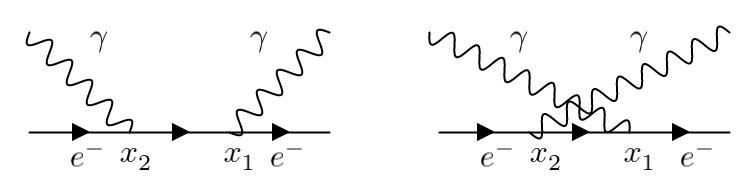
\includegraphics{Images/compton.png}
    \caption{Process (a) on the left and process (b) on the right.}
    \labfig{compton}
\end{figure}

In order to obtain that, we have to select from $S^{(2)}$ matrix elements that give us a meaningful result:
\begin{enumerate}[label=\alph*)]
    \item $\slashed{A}^+_2$ and $\Psi^+_2$ annihilate a photon and an electron in $x_2$, we have a fermion propagator that goes to $x_1$ where $\slashed{A}^-_1$ and $\Psi^-_1$ create an electron and a photon;
    \item in $x_2$, $\slashed{A}^-_2$ creates a photon while $\Psi^+_2$ annihilates an electron. Then we have the propagator going to $x_1$ where $\slashed{A}^+_1$ annihilates a photon and $\Psi^-_1$ creates an electron.
\end{enumerate}
The total amplitude of the Compton scattering is hence given by $S^{(2)}_a+S^{(2)}_b$:
\[
\left\{
\begin{aligned}
S_a^{(2)}&=(-ie)^2\int d^4x_1d^4x_2\norder{(\bar{\Psi}_1^-\slashed{A}_1^-)iS_F(x_1-x_2)(\slashed{A}_2^+\Psi_2^+)}\\
S_b^{(2)}&=(-ie)^2\int d^4x_1d^4x_2\norder{(\bar{\Psi}_1^-\slashed{A}_1^+)iS_F(x_1-x_2)(\slashed{A}_2^-\Psi_2^+)}
\end{aligned}
\right.
\Rightarrow S^{(2)}(\gamma e^-\xrightarrow[]{}\gamma e^-)=S_a^{(2)}+S_b^{(2)}
\]
\subsection{Bhabha scattering}
For the Bhabha scattering, we have that the second order S-matrix is given by:
\begin{align*}
S^{(2)}&=\frac{(-ie)^2}{2}\int d^4x_1d^4x_2\norder{\bar{\Psi}_1\gamma^\mu\Psi_1i\eta_{\mu\nu}D(x_1-x_2)\bar{\Psi}_2\gamma^\nu\Psi_2}\\
&=\frac{(-ie)^2}{2}\int d^4x_1d^4x_2\norder{(\bar{\Psi}_1^-+\bar{\Psi}_1^+)\gamma^\mu(\Psi_1^-+\Psi_1^+)i\eta_{\mu\nu}D(x_1-x_2)(\bar{\Psi}_2^-+\bar{\Psi}_2^+)\gamma^\nu(\Psi_2^-+\Psi_2^+)}
\end{align*}
What we want is $\ket{i}=\ket{e^+e^-}$ and $\ket{f}=\ket{e^+e^-}$:
\begin{figure}[h!]
    \centering
    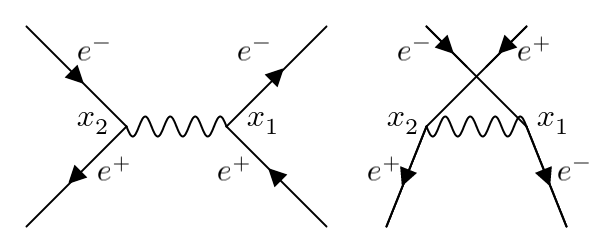
\includegraphics{Images/bhabha.png}
    \caption{Process (a) on the left and process (b) on the right. The arrows for the positrons are already inverted, i.e. a positron coming in has the arrow pointing outside and vice-versa. We will see why later.}
    \labfig{bhabha}
\end{figure}

As seen for Compton scattering, we have different objects contributing to this process:
\begin{enumerate}[label=\alph*)]
\item in $x_2$, a positron and an electron get annihilated, the photon propagator goes to $x_1$ where a positron and an electron are created;
\item the other possibility is to create and annihilate a positron in $x_2$ and an electron in $x_1$. 
\end{enumerate}
We have two other possibilities not shown in the picture, i.e. (a) and (b) but with the vertices reversed. This means just swapping $x_1$ and $x_2$, therefore they will give us the same contribution in the integral and we can erase the factor $1/2$:
\[
\left\{
\begin{aligned}
S_a^{(2)}&=(-ie)^2\int d^4x_1d^4x_2\norder{\bar{\Psi}_1^-\gamma^\mu\Psi_1^-i\eta_{\mu\nu}D(x_1-x_2)\bar{\Psi}_2^+\gamma^\nu\Psi_2^+}\\
S_b^{(2)}&=(-ie)^2\int d^4x_1d^4x_2\norder{\bar{\Psi}_1^-\gamma^\mu\Psi_1^+i\eta_{\mu\nu}D(x_1-x_2)\bar{\Psi}_2^+\gamma^\nu\Psi_2^-}
\end{aligned}
\right.
\Rightarrow S^{(2)}(e^+e^-\xrightarrow[]{}e^+e^-)=S_a^{(2)}+S_b^{(2)}
\]
\section{Feynman rules}
\labsec{frules}
Let's now consider the process $e^-\xrightarrow[]{}e^-\gamma$. Even if it is not physical, we just want to understand how the operators act, then we will move to a physical process. What we want to evaluate is $\bra{f}S^{(1)}\ket{i}$:\marginnote{}
\[
\begin{cases}
\ket{i}=\ket{e^-(p)}\\
\ket{f}=\ket{e^-(p'),\gamma(k)}
\end{cases}
\quad
\bra{f}S^{(1)}\ket{i}=-ie\int d^4x\bra{\tikzmark{startb1}e^-\tikzmark{startb2}\gamma}\tikzmark{endb1}\bar{\Psi}^-(x)\tikzmark{endb2}\slashed{A}^-(x)\tikzmark{startb3}\Psi^+(x)\ket{\tikzmark{endb3}e^-}
\begin{tikzpicture}[remember picture,overlay,line width=0.5pt]
\JoinDownF{(5pt,-1pt)}{(5pt,-1pt)}{b1}
\JoinUpF{(5pt,10pt)}{(5pt,10pt)}{b2}
\JoinDownF{(5pt,-1pt)}{(5pt,-1pt)}{b3}
\end{tikzpicture}
\]
Notice that \tikzmark{startp2}A\qquad\tikzmark{endp2}B is \textbf{not} a contraction, it is just to help visualizing which field annihilates/creates which particle.
\begin{tikzpicture}[remember picture,overlay,line width=0.5pt]
\JoinUpF{(5pt,8pt)}{(5pt,8pt)}{p2}
\end{tikzpicture}


Focusing now on the term $\Psi^+(x)\ket{e^-(p,n)}$:
\begin{align*}
\Psi^+(x)\ket{e^-(p',n')}&=\sum_{\pm n}\int\frac{d^3p}{(2\pi)^{3/2}}\sqrt{\frac{m}{E_p}}e^{-iP_\mu x^\mu}u(p,n)b(p,n)b^\dagger(p',n')\ket{0}\marginnote{$bb^\dagger=\delta(\underline{p}-\underline{p}')\delta_{nn'}-b^\dagger b$}\\
&=\sum_{\pm n}\int\frac{d^3p}{(2\pi)^{3/2}}\sqrt{\frac{m}{E_p}}u(p,n)\delta(\underline{p}-\underline{p}')\delta_{nn'}e^{-iP_\mu x^\mu}\ket{0}\\
&=\frac{1}{(2\pi)^{3/2}}\sqrt{\frac{m}{E_{p'}}}u(p',n')e^{-iP'_\mu x^\mu}\ket{0}\\
&=\sqrt{\frac{m}{VE_{p'}}}u(p',n')e^{-iP'_\mu x^\mu}\ket{0}
\end{align*}
The $V$ comes from the quantization in a \textbf{finite volume}, sending $1/(2\pi)^{3/2}$ to $1/\sqrt{V}$. With an analogous process, we can find that for $A_\mu^+(x)$ we have:
\[
A_\mu^+(x)\ket{\gamma(k,\lambda)}=\dots=\frac{1}{\sqrt{2E_kV}}\varepsilon_\mu^{(\lambda)}(k)e^{-iK_\mu x^\mu}\ket{0}
\]
In this way, the first order S-matrix can be re-written as:
\begin{align*}
\bra{f}S^{(1)}\ket{i}&={\color{red}-ie}\int d^4x\sqrt{\frac{m}{VE_{p'}}}\sqrt{\frac{m}{VE_p}}\frac{1}{\sqrt{2E_{k'}V}}{\color{blue}e^{iP'_\mu x^\mu}e^{iK_\mu x^\mu}e^{-iP_\mu x^\mu}}{\color{red}\bar{u}(p')\varepsilon_\mu^{(\lambda)}(k')\gamma^\mu u(p)}\\
&=(2\pi)^4{\color{blue}\delta(P'+K'-P)}\frac{m}{V}\frac{1}{\sqrt{2E_{p'}E_{k'}E_pV}}{\color{red}\pazocal{M}}
\end{align*}
This gives us the first \textbf{Feynman rules}:
\begin{kaobox}[frametitle=Feynman rules]
\[
\begin{aligned}
&\bullet\text{Incoming particle: } \sqrt{\frac{m}{VE_p}}u(p,n)\\
&\bullet\text{Outgoing particle: } \sqrt{\frac{m}{VE_{p'}}}\bar{u}(p',n')\\
&\bullet\text{Incoming/outgoing photon: } \frac{1}{\sqrt{2E_kV}}\varepsilon_\mu^{(\lambda)}(k)\\
&\bullet\text{Interaction vertex: } -ie\gamma^\mu
\end{aligned}
\]
\end{kaobox}
An additional rule is given by the way we wrote $\pazocal{M}$:
\[
\pazocal{M}=\bar{u}(p')(-ie\gamma^\mu)u(p)\varepsilon^{(\lambda)}_\mu(k')
\]
For \textbf{particles}, we put the final state first, then the interaction vertex and at the end the initial state. Moreover, the $\delta$ gives us the conservation of the total four-momentum. 

Moving to the second order, we consider now a \textbf{physical process}: Compton scattering, $e^-\gamma\xrightarrow[]{}e^-\gamma$ [\reffig{compton}].
\[
\begin{cases}
\ket{i}=\ket{e^-(p),\gamma(k)}\\
\ket{f}=\ket{e^-(p'),\gamma(k')}
\end{cases}
\quad
\bra{f}S_a^{(2)}\ket{i}=(-ie)^2\int d^4x_1d^4x_2\bra{\tikzmark{startc1}e^-\tikzmark{startc2}\gamma}\tikzmark{endc1}\bar{\Psi}^-_{x_1}\gamma^\mu\tikzmark{endc2}A^-_{\mu x_1} iS_F(x_1-x_2)\gamma^\nu\tikzmark{startc3}\Psi^+_{x_2}\tikzmark{startc4}A^+_{\nu x_2}\ket{\tikzmark{endc3}e^-\tikzmark{endc4}\gamma}
\begin{tikzpicture}[remember picture,overlay,line width=0.5pt]
\JoinUpF{(5pt,10pt)}{(5pt,10pt)}{c1}
\JoinDownF{(5pt,-1pt)}{(5pt,-1pt)}{c2}
\JoinUpF{(5pt,10pt)}{(5pt,10pt)}{c3}
\JoinDownF{(5pt,-1pt)}{(5pt,-1pt)}{c4}
\end{tikzpicture}
\]
The propagator $iS_F(x)$ can be written as:
\[
iS_F(x)=\int\frac{d^4p}{(2\pi)^4}e^{-iP_\mu x^\mu}i\Tilde{S}_F(p) \quad \text{with } \Tilde{S}_F(p)=\frac{\slashed{P}+m}{P^2-m^2+i\varepsilon}
\]
Substituting this in the second order matrix computed above and keeping in mind the first Feynman rules we computed, gives us:
\begin{align*}
\bra{f}S_a^{(2)}\ket{i}&=(-ie)^2\int d^4x_1d^4x_2\sqrt{\frac{m}{VE_{p'}}}\sqrt{\frac{m}{VE_p}}\frac{1}{\sqrt{2VE_{k'}}}\frac{1}{\sqrt{2VE_k}}\bar{u}(p')\gamma^\mu\varepsilon^{(\lambda)}_\mu(k')e^{iP'_\mu x_1^\mu}e^{iK'_\mu x_1^\mu}\\
&\times\frac{i}{(2\pi)^4}\int d^4qe^{-iQ_\mu(x_1-x_2)^\mu}\Tilde{S}_F(q)u(p)\gamma^\nu\varepsilon^{(\lambda)}_\nu(k)e^{-iP_\mu x_2^\mu}e^{-iK_\mu x_2^\mu}\\
&=\prod_{\text{fer}}\sqrt{\frac{m}{VE_f}}\prod_{\text{bos}}\frac{1}{\sqrt{2VE_b}}\int d^4x_1d^4x_2\\
&\times\int\frac{d^4q}{(2\pi)^4}{\color{blue}e^{i(P'+K')_\mu x_1^\mu}}{\color{green}e^{-i(P+K)_\mu x_2^\mu}}{\color{blue}e^{-iQ_\mu x_1^\mu}}{\color{green}e^{iQ_\mu x_2^\mu}}{\color{red}\bar{u}(p')(-ie\gamma^\mu)\varepsilon^{(\lambda)}_\mu(k)\frac{i}{\slashed{Q}-m+i\varepsilon}(-ie\gamma^\nu)\varepsilon^{(\lambda)}_\nu(k)u(p)}\\
&=\prod_{\text{fer}}\sqrt{\frac{m}{VE_f}}\prod_{\text{bos}}\frac{1}{\sqrt{2VE_b}}\int\frac{d^4q}{(2\pi)^4}{\color{blue}\delta(P'+K'-Q)}(2\pi)^4{\color{green}\delta(Q-P-K)}{\color{red}\pazocal{M}_a}\\
&=\prod_{\text{fer}}\sqrt{\frac{m}{VE_f}}\prod_{\text{bos}}\frac{1}{\sqrt{2VE_b}}(2\pi)^4\delta(P'+K'-P-K)\pazocal{M}_a
\end{align*}
$Q=P+K$ and the complete expression for $\pazocal{M}_a$ is:
\[
\pazocal{M}_a=\bar{u}(p')(-ie\gamma^\mu)\varepsilon^{(\lambda)}_\mu(k')\frac{i}{(\slashed{P}+\slashed{K})-m+i\varepsilon}(-ie\gamma^\nu)\varepsilon_\nu^{(\lambda)}(k)u(p)
\]
With the same reasoning, keeping in mind that now $Q=P-K'$, for $S_b^{(2)}$ we get:
\[
\pazocal{M}_b=\bar{u}(p')(-ie\gamma^\mu)\varepsilon^{(\lambda)}_\mu(k)\frac{i}{(\slashed{P}-\slashed{K}')-m+i\varepsilon}(-ie\gamma^\nu)\varepsilon_\nu^{(\lambda)}(k')u(p)
\]
The full expression of $\bra{f}S^{(2)}\ket{i}$ is therefore:
\[
\bra{f}S^{(2)}\ket{i}=\prod_{\text{fer}}\sqrt{\frac{m}{VE_f}}\prod_{\text{bos}}\frac{1}{\sqrt{2VE_b}}(2\pi)^4\delta(P'+K'-P-K)(\pazocal{M}_a+\pazocal{M}_b)
\]
This gives us the Feynman rule for the fermionic propagator:
\begin{kaobox}[frametitle=Feynman rules]
\[
\bullet\text{Fermionic propagator: }\; \frac{i}{\slashed{Q}-m+i\varepsilon}
\]
\end{kaobox}
\begin{marginfigure}
    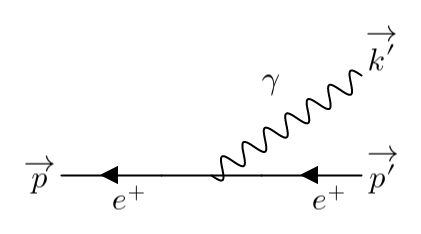
\includegraphics{Images/positron.png}
    \caption{Positron scattering}
    \labfig{positron}
\end{marginfigure}
What happens when we have \textbf{anti-particles}, e.g. a positron?
\[
\begin{cases}
\ket{i}=\ket{e^+(p)}\\
\ket{f}=\ket{e^+(p'),\gamma(k')}
\end{cases}
\quad 
\bra{f}S^{(1)}\ket{i})=-ie\int d^4x\bra{\tikzmark{startd1}e^+\tikzmark{startd2}\gamma}\tikzmark{startd3}\bar{\Psi}^+\tikzmark{endd2}\slashed{A}^-\tikzmark{endd1}\Psi^-\ket{\tikzmark{endd3}e^+}
\begin{tikzpicture}[remember picture,overlay,line width=0.5pt]
\JoinDownF{(5pt,-5pt)}{(5pt,-5pt)}{d1}
\JoinDownF{(5pt,-1pt)}{(5pt,-1pt)}{d2}
\JoinUpF{(5pt,10pt)}{(5pt,10pt)}{d3}
\end{tikzpicture}
\]
Computing this gives us additional Feynman rules for anti-particles:
\begin{align*}
\bra{f}S^{(1)}\ket{i}&={\color{red}-ie}\int d^4x\sqrt{\frac{m}{VE_{p'}}}\sqrt{\frac{m}{VE_p}}\frac{1}{\sqrt{2VE_{k'}}}{\color{blue}e^{iP'_\mu x^\mu}e^{iK'_\mu x^\mu}e^{-iP_\mu x^\mu}}{\color{red}\bar{v}(p')\gamma^\mu\varepsilon_\mu^{(\lambda)}(k')v(p)}\\
&=(2\pi)^4{\color{blue}\delta(P'+K'-P)}\frac{m}{V}\frac{1}{\sqrt{2E_{p'}E_{k'}E_pV}}{\color{red}\pazocal{M}}
\end{align*}
The Feynman rules we obtain from this process are:
\begin{kaobox}[frametitle=Feynman rules]
\[
\begin{aligned}
&\bullet\text{Incoming anti-particle: }\; \sqrt{\frac{m}{VE_p}}\bar{v}(p,n)\\
&\bullet\text{Outgoing anti-particle: }\; \sqrt{\frac{m}{VE_{p'}}}v(p',n')\\
\end{aligned}
\]
\end{kaobox}
The reading order of $\pazocal{M}$ is the same as the one we obtained for particles:
\[
\pazocal{M}=\bar{v}(p')(-ie\gamma^\mu)v(p)\varepsilon^{(\lambda)}_\mu(k')
\]
{\fontencoding{U}\fontfamily{futs}\selectfont\char 66\relax}
In order to use the same rules for particles, for anti-particles the arrows are \textbf{inverted} [\reffig{positron}]: the incoming positron has the arrow pointing outside while the outgoing positron has the arrow pointing inside.
The last thing left to compute is the \textbf{electron self-energy}:
\[
\bra{f}S^{(2)}\ket{i}&=(-ie)^2\int d^4x_1d^4x_2\bra{\tikzmark{starte1}e^-}\tikzmark{ende1}\bar{\Psi}_{x_1}^-\gamma_\mu iS_F(x_1-x_2)i\eta_{\mu\nu}D(x_1-x_2)\gamma_\nu\tikzmark{starte2}\Psi_{x_2}^+\ket{\tikzmark{ende2}e^-}
\]
\begin{tikzpicture}
[remember picture,overlay,line width=0.5pt]
\JoinDownF{(5pt,-1pt)}{(5pt,-1pt)}{e1}
\JoinDownF{(5pt,-1pt)}{(5pt,-1pt)}{e2}
\end{tikzpicture}
\begin{marginfigure}
    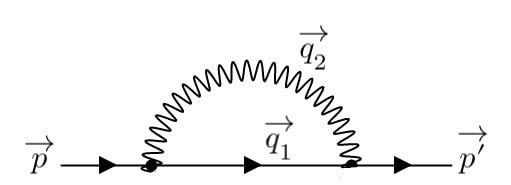
\includegraphics{Images/selfenergy.jpg}
    \caption{Electron self-energy}
    \labfig{selfenergy}
\end{marginfigure}
As we did for the propagator $iS_F(x)$, we can rewrite $i\eta_{\mu\nu}D(x)$:
\[
i\eta_{\mu\nu}D(x)=\int\frac{d^4p}{(2\pi)^4}e^{-iPx}i\eta_{\mu\nu}\Tilde{D}(p) \quad \text{with } \Tilde{D}(p)=-\frac{1}{P^2+i\varepsilon}
\]
With this substitution, the second order matrix becomes:
\begin{align*}
\bra{f}S^{(2)}\ket{i}&=\sqrt{\frac{m}{VE_p}}\sqrt{\frac{m}{VE_{p'}}}\int d^4x_1d^4x_2e^{iP'_\mu x_1^\mu}\bar{u}(p')(-ie\gamma_\mu)\\
&\times\int\frac{d^4q_1}{(2\pi)^4}e^{-iQ_{1\mu}(x_1-x_2)^\mu}i\Tilde{S}_F(q_1)(-ie\gamma_\nu)\\
&\times\int\frac{d^4q_2}{(2\pi)^4}e^{-iQ_{2\mu}(x_1-x_2)^\mu}i\eta_{\mu\nu}\Tilde{D}(q_2)e^{-iP_\mu x_2^\mu}u(p)\\
&=\sqrt{\frac{m}{VE_p}}\sqrt{\frac{m}{VE_{p'}}}\int\frac{d^4q_1}{(2\pi)^4}\int\frac{d^4q_2}{(2\pi)^4}\delta(P'-Q_1-Q_2)\delta(Q_1+Q_2-P)\\
&\times{\color{red}\bar{u}(p')(-ie\gamma_\mu)\frac{i}{\slashed{Q_1}-m+i\varepsilon}(-ie\gamma_\nu)\frac{(-i\eta_{\mu\nu})}{Q_2^2+i\varepsilon}u(p)}\\
&=\sqrt{\frac{m}{VE_p}}\sqrt{\frac{m}{VE_{p'}}}\delta(P'-P)(2\pi)^4{\color{red}\pazocal{M}} 
\end{align*}
Where we denoted with $\pazocal{M}$ the term:
\[
\pazocal{M}=\int\frac{d^4q_2}{(2\pi)^4}\bar{u}(p')(-ie\gamma_\mu)\frac{i}{(\slashed{P}-\slashed{Q_2})-m+i\varepsilon}(-ie\gamma_\nu)\frac{(-i\eta_{\mu\nu})}{Q_2^2+i\varepsilon}u(p)
\]
This gives us an additional Feynman rule:
\begin{kaobox}[frametitle=Feynman rules]
\[
\text{Virtual photon: }\quad \frac{-i\eta_{\mu\nu}}{K^2+i\varepsilon}
\]
\end{kaobox}
\section{Production cross section}
Moving to a probability, what we want to study is now:
\[
|S_{fi}|^2=|(2\pi)^4\delta^4(\sum_iP_i^{ext})|^2\prod_{\text{fer}}\frac{m}{VE_p}\prod_{\text{bos}}\frac{1}{2VE_b}|\pazocal{M}|^2
\]
The term with the $\delta$ function can be rewritten as:
\[
(2\pi)^4\delta^4(P_f-P_i)=\lim_{V\to\infty\\T\to\infty}\int_V d^3x\int_{-T/2}^{+T/2}dte^{i(P_f-P_i)x}
\]
Focusing for the moment on the integration over time:
\[
(2\pi)^4\delta(E_f-E_i)=\lim_{T\to\infty}\int_{-T/2}^{+T/2}dte^{i\Delta Et}=\lim_{T\to\infty}\frac{2\sin(\Delta ET/2)}{\Delta E}
\]
\[
\lim_{T\to\infty}\frac{4\sin^2(\Delta ET/2)}{\Delta E^2}\sim2\pi T\delta(E_f-E_i)
\]
where we computed the square of this quantity because this is what we are interested in. We can do the same for the integration in $d^3x$ over a volume $V$ and what we get at the end is:
\[
|(2\pi)^4\delta^4(P_f-P_i)|^2=\lim_{V\to\infty\\T\to\infty}(2\pi)^4VT\delta^4(P_f-P_i)
\]
At this point we define the \textbf{transition rate} as:
\[
\omega_{fi}:=\frac{|S_{fi}|^2}{T}=V(2\pi)^4\delta^4(P_f-P_i)\underbrace{\prod_{\text{fer}}\frac{1}{2VE_p}\prod_{\text{bos}}\frac{1}{2VE_b}}_{\big{\prod_{\text{ext}}\frac{1}{2EV}}}\prod_{\text{fer}}2m_f|\pazocal{M}|^2
\]
This is the transition probability density per unit time to go from an initial state $p_i$ to an exact final state $p_f$. However, we are not usually able to get exactly $p_f$ so we take into account the possibility to have a final state in $[p_f,p_f+dp_f]$. We are going to sum over all the possible final states inside the interval $dp_f$: how many are they? We have to move from $dp$ to $dn$. We know that the momentum is quantized:
\[
\underline{p}=\frac{2\pi}{L}\underline{n}\xrightarrow[]{}d^3n=\frac{L^3}{(2\pi)^3}d^3p_f
\]
Therefore the object we want to study is:
\[
\omega_{fi}\prod_f\frac{L^3}{(2\pi)^3}d^3p_f
\]
To define the cross section, we first need to define some quantities:
\[
\begin{cases}
n: \text{\# of incoming particles per unit time and surface}\\
N_i: \text{\# of incoming particles in $\Delta t\Rightarrow N_i=nS\Delta t$}\\
N: \text{\# of scattered particles per unit time and unit target}\\
N_d: \text{\# of scattered particles in $\Delta t\Rightarrow N_d=N\Delta t$}
\end{cases}
\]
The cross section $\sigma$ can be expressed as:
\[
\sigma=\frac{N}{n}=\frac{N_d}{\Delta t}\frac{S\Delta t}{N_i}=\frac{N_d}{N_i}S
\]
$n$ is the flux of incoming particles, which means:
\[
n=\frac{N_i}{{\color{red}S}{\color{green}\Delta t}}\frac{{\color{green}L}}{{\color{red}L}}=\frac{N_i}{{\color{red}V}}{\color{green}v_{rel}}=\rho|\underline{v}_{rel}|
\]
Putting everything together, we obtain the \textbf{differential cross section}:
\begin{align*}
d\sigma&=\frac{dN}{n}=\frac{dN}{\rho|\underline{v}|}=\omega_{fi}\prod_f\frac{V}{(2\pi)^3}d^3p_f\frac{1}{\rho|\underline{v}|}\marginnote{We consider one scattering at a time, so $\rho=1/V$.}\\
&=\frac{V^2}{|\underline{v}|}(2\pi)^4\delta^4(P_f-P_i)\prod_{\text{ext}}\frac{1}{2EV}\prod_{\text{fer}}2m_f|\pazocal{M}|^2\prod_{\text{f}}\frac{V}{(2\pi)^3}d^3p_f
\end{align*}
Considering now the case of 2 particles, i.e. bullet and fixed target, going into $n$ final ones:
\begin{equation}
\labeq{dsigma}
d\sigma=\frac{(2\pi)^4}{|\underline{v}|}\delta^4(P_f-P_i)\frac{1}{4E_1E_2}\prod_{\text{fer}}2m_f\prod_{\text{f}}\frac{d^3p_f}{(2\pi)^3}\frac{1}{2E_f}|\pazocal{M}|^2
\end{equation}
We explicitly write the relative velocity as:
\[
\left\{
\begin{aligned}
&\underline{v}=\underline{v}_1-\underline{v}_2=\frac{p_1}{E_1}-\frac{p_2}{E_2}\\
&E_1E_2|\underline{v}|=E_1E_2|\underline{v}_1-\underline{v}_2|=\left|\frac{p_1}{E_1}-\frac{p_2}{E_2}\right|E_1E_2
\end{aligned}
\right.
\]
We are studying a fixed target experiment, therefore $P_2^\mu=(m_2,\underline{0})$ and $\underline{v}=\underline{v}_1$:
\[
E_1E_2|\underline{v}|=E_1m_2\frac{|p_1|}{E_1}=m_2|p_1|=m_2\sqrt{E_1^2-m_1^2}=\sqrt{m_2^2E_1^2-m_1^2m_2^2}=\sqrt{(P_1\cdot P_2)^2-m_1^2m_2^2}
\]
This is invariant, we know the other objects in \refeq{dsigma} are invariant therefore the differential cross section $d\sigma$ is an invariant object.
\subsection{Scattering $e^+e^-\xrightarrow[]{}\mu^+\mu^-$}
\marginnote{This section is based on \cite{scattering}.}
Consider now the process $e^+e^-\xrightarrow[]{}\mu^+\mu^-$, \refeq{dsigma} now becomes:
\[
d\sigma=(2\pi)^4\delta^4(P_1+P_2-P_3-P_4)\frac{1}{4\sqrt{(P_1\cdot P_2)^2-m_e^2m_e^2}}(2m_e)^2(2m_e)^2\frac{d^3p_3}{(2\pi)^3}\frac{1}{2E_3}\frac{d^3p_4}{(2\pi)^3}\frac{1}{2E_4}|\pazocal{M}|^2
\]
The interaction Lagrangian is given by:
\[
\pazocal{L}_{int}=-e\norder{\left[\bar{\Psi}_e\slashed{A}\Psi_e+\bar{\Psi}_\mu\slashed{A}\Psi_\mu\right]}
\]
We take the second order contribution, which is the first one with a physical sense and we obtain:
\[
S^{(2)}=\frac{(-ie)^2}{2}\int d^4x_1d^4x_2T\left[\left(\norder{\bar{\Psi}_e\slashed{A}\Psi_e+\bar{\Psi}_\mu\slashed{A}\Psi_\mu}\right)_1\left(\norder{\bar{\Psi}_e\slashed{A}\Psi_e+\bar{\Psi}_\mu\slashed{A}\Psi_\mu}\right)_2\right]
\]
We ignore terms involving $e^+e^-\xrightarrow[]{}e^+e^-$ and $\mu^+\mu^-\xrightarrow[]{}\mu^+\mu^-$ and we get:
\[
S^{(2)}=\frac{(-ie)^2}{2}\int d^4x_1d^4x_2T\left[\left(\norder{\bar{\Psi}_e\tikzmark{startd1}\slashed{A}\Psi_e}\right)_1\left(\norder{\bar{\Psi}_\mu\tikzmark{endd1}\slashed{A}\Psi_\mu}\right)_2+\left(\norder{\bar{\Psi}_\mu\tikzmark{startd2}\slashed{A}\Psi_\mu}\right)_1\left(\norder{\bar{\Psi}_e\tikzmark{endd2}\slashed{A}\Psi_e}\right)_2\right]
\begin{tikzpicture}[remember picture,overlay,line width=0.5pt]
\JoinUp{(5pt,10pt)}{(5pt,10pt)}{d1}
\JoinUp{(5pt,10pt)}{(5pt,10pt)}{d2}
\end{tikzpicture}
\]
This object corresponds to:
\begin{figure}[h!]
    \centering
    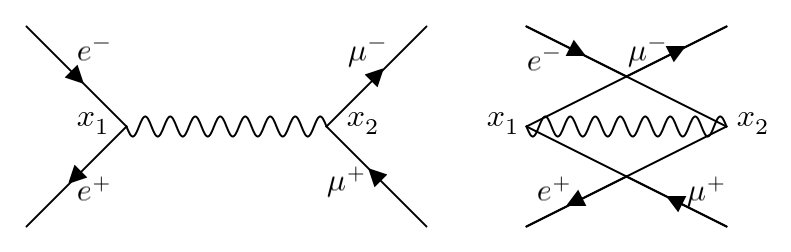
\includegraphics{Images/feynman.png}
    \caption*{}
    \labfig{fig:my_label}
\end{figure}

What we want to calculate at the end is the S-matrix. Since the process on the right can be obtained by exchanging $x_1$ and $x_2$ in the process on the left, the contribution to this scattering is twice the matrix element, therefore:
\[
S_{fi}=(-ie)^2\int d^4x_1d^4x_2\bra{\mu^+\mu^-}\norder{\bar{\Psi}_e(x_1)\Psi_e(x_1)\gamma^\mu i\eta_{\mu\nu}D(x_1-x_2)\gamma^\nu\bar{\Psi}_\mu(x_2)\Psi_\mu(x_2)}\ket{e^+e^-}
\]
As we said we focus just on the diagram on the left and, using the Feynman rules we found in \refsec{frules}, we can write the transition amplitude as:\begin{marginfigure}
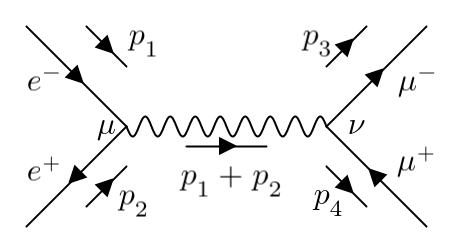
\includegraphics{Images/feynman(5).png}
\end{marginfigure}
\begin{align*}
\pazocal{M}&=\bar{u}_i(p_3)(-ie\gamma^\nu)_{ij}v_j(p_4)\frac{(-i\eta_{\mu\nu})}{(P_1+P_2)^2}\bar{v}_k(p_2)(-ie\gamma^\mu)_{kl}u_l(p_1)\\
&=\frac{ie^2}{(P_1+P_2)^2}\bar{u}_{3i}\gamma^{\nu ij}v_{4j}\bar{v}_{2k}\gamma^\nu_{kl}u_{1l}
\end{align*}
But what we are interested in is the modulus squared of this object, i.e. $|\pazocal{M}|^2=\pazocal{M}\pazocal{M}^\dagger$:
\[
\pazocal{M}^\dagger=\frac{-ie^2}{(P_1+P_2)^2}\bar{v}_{4j}\gamma_{\mu ji}u_{3i}\bar{u}_{1l}\gamma^\mu_{lk}v_{2k}
\]
\begin{align*}
|\pazocal{M}|^2&=\frac{e^4}{(P_1+P_2)^4}\left[(\bar{u}_{3i}\gamma_{\nu ij}v_{4j}\bar{v}_{2k}\gamma^\nu_{kl}u_{il})(\bar{v}_{4j}\gamma_{\mu ji}u_{3i}\bar{u}_{1l}\gamma^\mu_{lk}v_{2k})\right]\\
&=\frac{e^4}{(P_1+P_2)^4}\left[(\bar{u}_{3i}\gamma_{\nu ij}\bar{v}_{4j}\bar{v}_{4j}\gamma_{\mu ji}u_{3i})(\bar{v}_{2k}\gamma^\nu_{kl}u_{1l}\bar{u}_{1l}\gamma^\mu_{lk}v_{2k})\right]
\end{align*}
We do not consider the polarization, therefore we have to sum over all the possible initial and final states and divide by four:
\[
|\overline{\pazocal{M}}|^2=\frac{1}{4}|\pazocal{M}|^2=\frac{e^4}{4(P_1+P_2)^4}\sum_{n_3n_4}(\bar{u}_{3i}\gamma_{\nu ij}\bar{v}_{4j}\bar{v}_{4j}\gamma_{\mu ji}u_{3i})\sum_{n_1n_2}(\bar{v}_{2k}\gamma^\nu_{kl}u_{1l}\bar{u}_{1l}\gamma^\mu_{lk}v_{2k})
\]
Keep in mind that for the two sums we already know:
\[
\left\{
\begin{aligned}
\sum_{n_1}u_1\bar{u}_1&=\frac{\slashed{P}_1+m_e}{2m_e} \quad \sum_{n_2}v_2\bar{v}_2=\frac{\slashed{P}_2-m_e}{2m_e}\\
\sum_{n_3}u_3\bar{u}_3&=\frac{\slashed{P}_3+m_\mu}{2m_\mu} \quad \sum_{n_4}v_4\bar{v}_4=\frac{\slashed{P}_4-m_\mu}{2m_\mu}
\end{aligned}
\right.
\]
With this substitution, the transition amplitude can be written as:
\[
|\overline{\pazocal{M}}|^2=\frac{e^4}{(P_1+P_2)^4}\tr\left[\frac{\slashed{P}_3+m_\mu}{2m_\mu}\gamma_\nu\frac{\slashed{P}_4-m_\mu}{2m_\mu}\gamma_\mu\right]\tr\left[\frac{\slashed{P}_2-m_e}{2m_e}\gamma^\nu\frac{\slashed{P}_1+m_e}{2m_e}\gamma^\mu\right]
\]
Let's focus for the moment on the first trace:
\[
\tr\left[(\slashed{P}_3+m_\mu)\gamma_\nu(\slashed{P}_4-m_\mu)\gamma_\mu\right]
\quad
\begin{cases}
\text{odd number of $\gamma$ matrices$\xrightarrow[]{}0$}\\
\text{even number of $\gamma$ matrices$\xrightarrow[]{}\neq0$}
\end{cases}
\]
\begin{align*}
\tr\left[(\slashed{P}_3+m_\mu)\gamma_\nu(\slashed{P}_4-m_\mu)\gamma_\mu\right]&=\dots=\tr\left[\slashed{P}_3\gamma_\nu\slashed{P}_4\gamma_\mu-m_\mu^2\gamma_\nu\gamma_\mu\right]\\
&=4(P_{3\nu}P_{4\mu})+4(P_{3\mu}P_{4\nu})-4(P_3P_4)\eta_{\mu\nu}-4m_\mu^2\eta_{\mu\nu}
\end{align*}
Analogously, for the second trace we get:
\[
\tr\left[(\slashed{P}_2-m_e)\gamma^\nu(\slashed{P}_1+m_e)\gamma^\mu\right]=4(P_{1\mu}P_{2\nu})+4(P_{1\nu}P_{2\mu})-4(P_1P_2)\eta_{\mu\nu}-4m_e^2\eta_{\mu\nu}
\]
Putting everything together, what we get in the end is:
\[
|\overline{\pazocal{M}}|^2=\frac{e^4}{2(P_1+P_2)^4}\frac{1}{m_\mu^2m_e^2}\left[(P_1P_3)(P_2P_4)+(P_1P_4)(P_2P_3)+m_e^2(P_3P_4)+m_\mu^2(P_1P_2)+2m_e^2m_\mu^2\right]
\]
We work in the center of mass frame, which means:\begin{marginfigure}
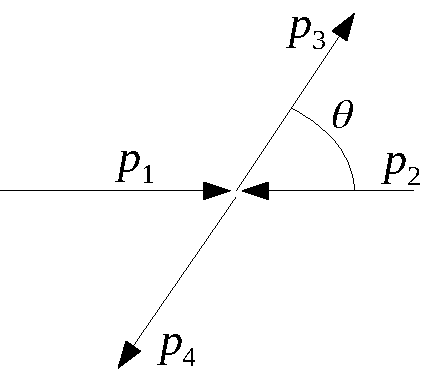
\includegraphics{Images/cdm.pdf}
\caption{Representation of what happens in the center of mass.}
\end{marginfigure}
\[
\left\{
\begin{aligned}
P_1^\mu&=(E_1,\underline{p}_1)\\
P_2^\mu&=(E_2,\underline{p}_2)
\end{aligned}
\right.
\quad
\left\{
\begin{aligned}
P_3^\mu&=(E_3,\underline{p}_3)\\
P_4^\mu&=(E_4,\underline{p}_4)
\end{aligned}
\right.
\]
Since $P_1^2=P_2^2=m_e^2$, this tells us that $E_1=E_2=E$, therefore $\underline{p_2}=-\underline{p_1}$. The same happens for $P_3$ and $P_4$: $\underline{p_4}=-\underline{p_3}$ and $E_3=E_4$. The conservation of energy tells us that:
\[
P_1+P_2=(2E,\underline{0})=P_3+P_4=(2E_3,\underline{0})\Rightarrow E_3=E_4=E
\]
\[
\left\{
\begin{aligned}
P_1^\mu&=(E,\underline{p})\\
P_2^\mu&=(E,-\underline{p})
\end{aligned}
\right.
\quad
\left\{
\begin{aligned}
P_3^\mu&=(E,\underline{p}')\\
P_4^\mu&=(E,-\underline{p}')
\end{aligned}
\right.
\]
It is now possible to compute the scalar products in the expression for the transition amplitude computed above:
\[
\left\{
\begin{aligned}
&(P_1P_2)=E^2+p^2 \quad (P_3P_4)=E^2+p'^2\\
&(P_1P_3)=(P_2P_4)=E^2-pp'\cos(\theta)\\
&(P_1P_4)=(P_2P_3)=E^2+pp'\cos(\theta)
\end{aligned}
\right.
\]
The transition amplitude now becomes:
\[
|\overline{\pazocal{M}}|^2=\frac{e^4}{2m_\mu^2m_e^216E^4}\left[(E^2-pp'\cos\theta)^2+(E^2+pp'\cos\theta)^2+m_e^2(E^2+p'^2)+m_\mu^2(E^2+p^2)+2m_e^2m_\mu^2\right]
\]
We know that $m_e=0.511$MeV$\ll m_\mu=105$MeV. With this approximation, we get:
\[
16m_e^2m_\mu^2|\overline{\pazocal{M}}|^2\simeq\frac{e^4}{2E^4}(2E^4+2E^2p'^2\cos^2\theta+2m_\mu^2E^2)=\frac{e^4}{E^2}(E^2+p'^2\cos^2\theta+m_\mu^2)
\]
The flux term in the cross section computed in the beginning becomes just $4\sqrt{(P_1\cdot P_2)^2-m_e^2m_\mu^2}\simeq8E^2$ and finally for the differential cross section we can write:
\begin{align*}
d\sigma&=(2\pi)^4\delta^4(P_f-P_i)\frac{e^4}{8E^4}(E^2+p'^2\cos^2\theta+m_\mu^2)\frac{d^3p_3}{(2\pi)^32E}\frac{d^3p_4}{(2\pi)^32E}\marginnote{$\delta(P_f-P_i)=\delta(E_1+E_2-E_3-E_4)=\delta(2E-2E')=\frac{1}{2}\delta(E-E')$}\\
&=\frac{e^4}{128\pi^2E^6}\delta(2E-2E')(E^2+p'^2\cos^2\theta+m_\mu^2)d^3p'
\end{align*}
Keeping in mind that $d^3p'=d\Omega dp'p'^2$, we can write:
\[
\frac{d\sigma}{d\Omega}=\frac{e^4}{128\pi^2E^6}\frac{1}{2}\int dp'p'^2(E^2+p'^2\cos^2\theta+m_\mu^2)\delta(E-E')
\]
In order to use the delta function, we write the momentum $p'$ in terms of the energy $E'$:
\[
p'^2=E'^2-m_\mu^2\xrightarrow[]{}\frac{dp'}{dE'}=\frac{E'}{p'}=\frac{E'}{\sqrt{E'^2-m_\mu^2}}
\]
Substituting this, we get:
\begin{align*}
\frac{d\sigma}{d\Omega}&=\frac{e^4}{128\pi^2E^6}\frac{1}{2}\int dE'\frac{E'}{p'}p'^2(E^2+p'^2\cos^2\theta+m_\mu^2)\delta(E-E')\\
&=\frac{e^4}{256\pi^2E^6}\int dE'E'\sqrt{E'^2-m_\mu^2}[E^2+(E'^2-m_\mu^2)\cos^2\theta+m_\mu^2]\delta(E-E')\\
&=\frac{e^4}{256\pi^2E^6}E\sqrt{E^2-m_\mu^2}(E^2+E^2\cos^2\theta+m_\mu^2-m_\mu^2\cos^2\theta)
\end{align*}
In the energy limit $E\gg m_\mu$, the expression above becomes:
\[
\frac{d\sigma}{d\Omega}\simeq\frac{e^4}{256\pi^2E^6}E^4(1+\cos^2\theta)=\frac{\alpha^2}{16E^2}(1+\cos^2\theta)
\]
Where we used the constant $\alpha=\frac{e^2}{4\pi}$. To conclude, we integrate over the angle to get the total cross section:
\[
\int_0^{2\pi}d\phi\int_{-1}^{+1}d\cos\theta(1+\cos^2\theta)=\frac{16\pi}{3}
\]
And finally we obtain:
\[
\sigma=\frac{\alpha^2\pi}{3E^2}\simeq5.6\cdot10^{-5}\frac{1}{E^2}
\]
This depends on the energy of the incoming particle. For instance, a beam of 100 GeV will give us a cross section of $\sigma\sim10^{-12}$ barn.
\newline
\begin{center}
So long, and thanks for all the fish\\
Addio, e grazie per tutto il pesce
\end{center}
\end{document}